\FloatBarrier
\section{Introduction}
\label{sec:intro}

I chose to address prompt 1, ``create and test an object/device that addresses a need or problem in your field of study,'' for my final project. I created a mock satellite with a solar panel and a sun sensor. The satellite rotates on two axes to point its solar panel in the direction of the sun as detected by the sun sensor. The completed build is shown in Figure~\ref{fig:satellite-completed}.
\begin{figure}[!ht]
    \centering
    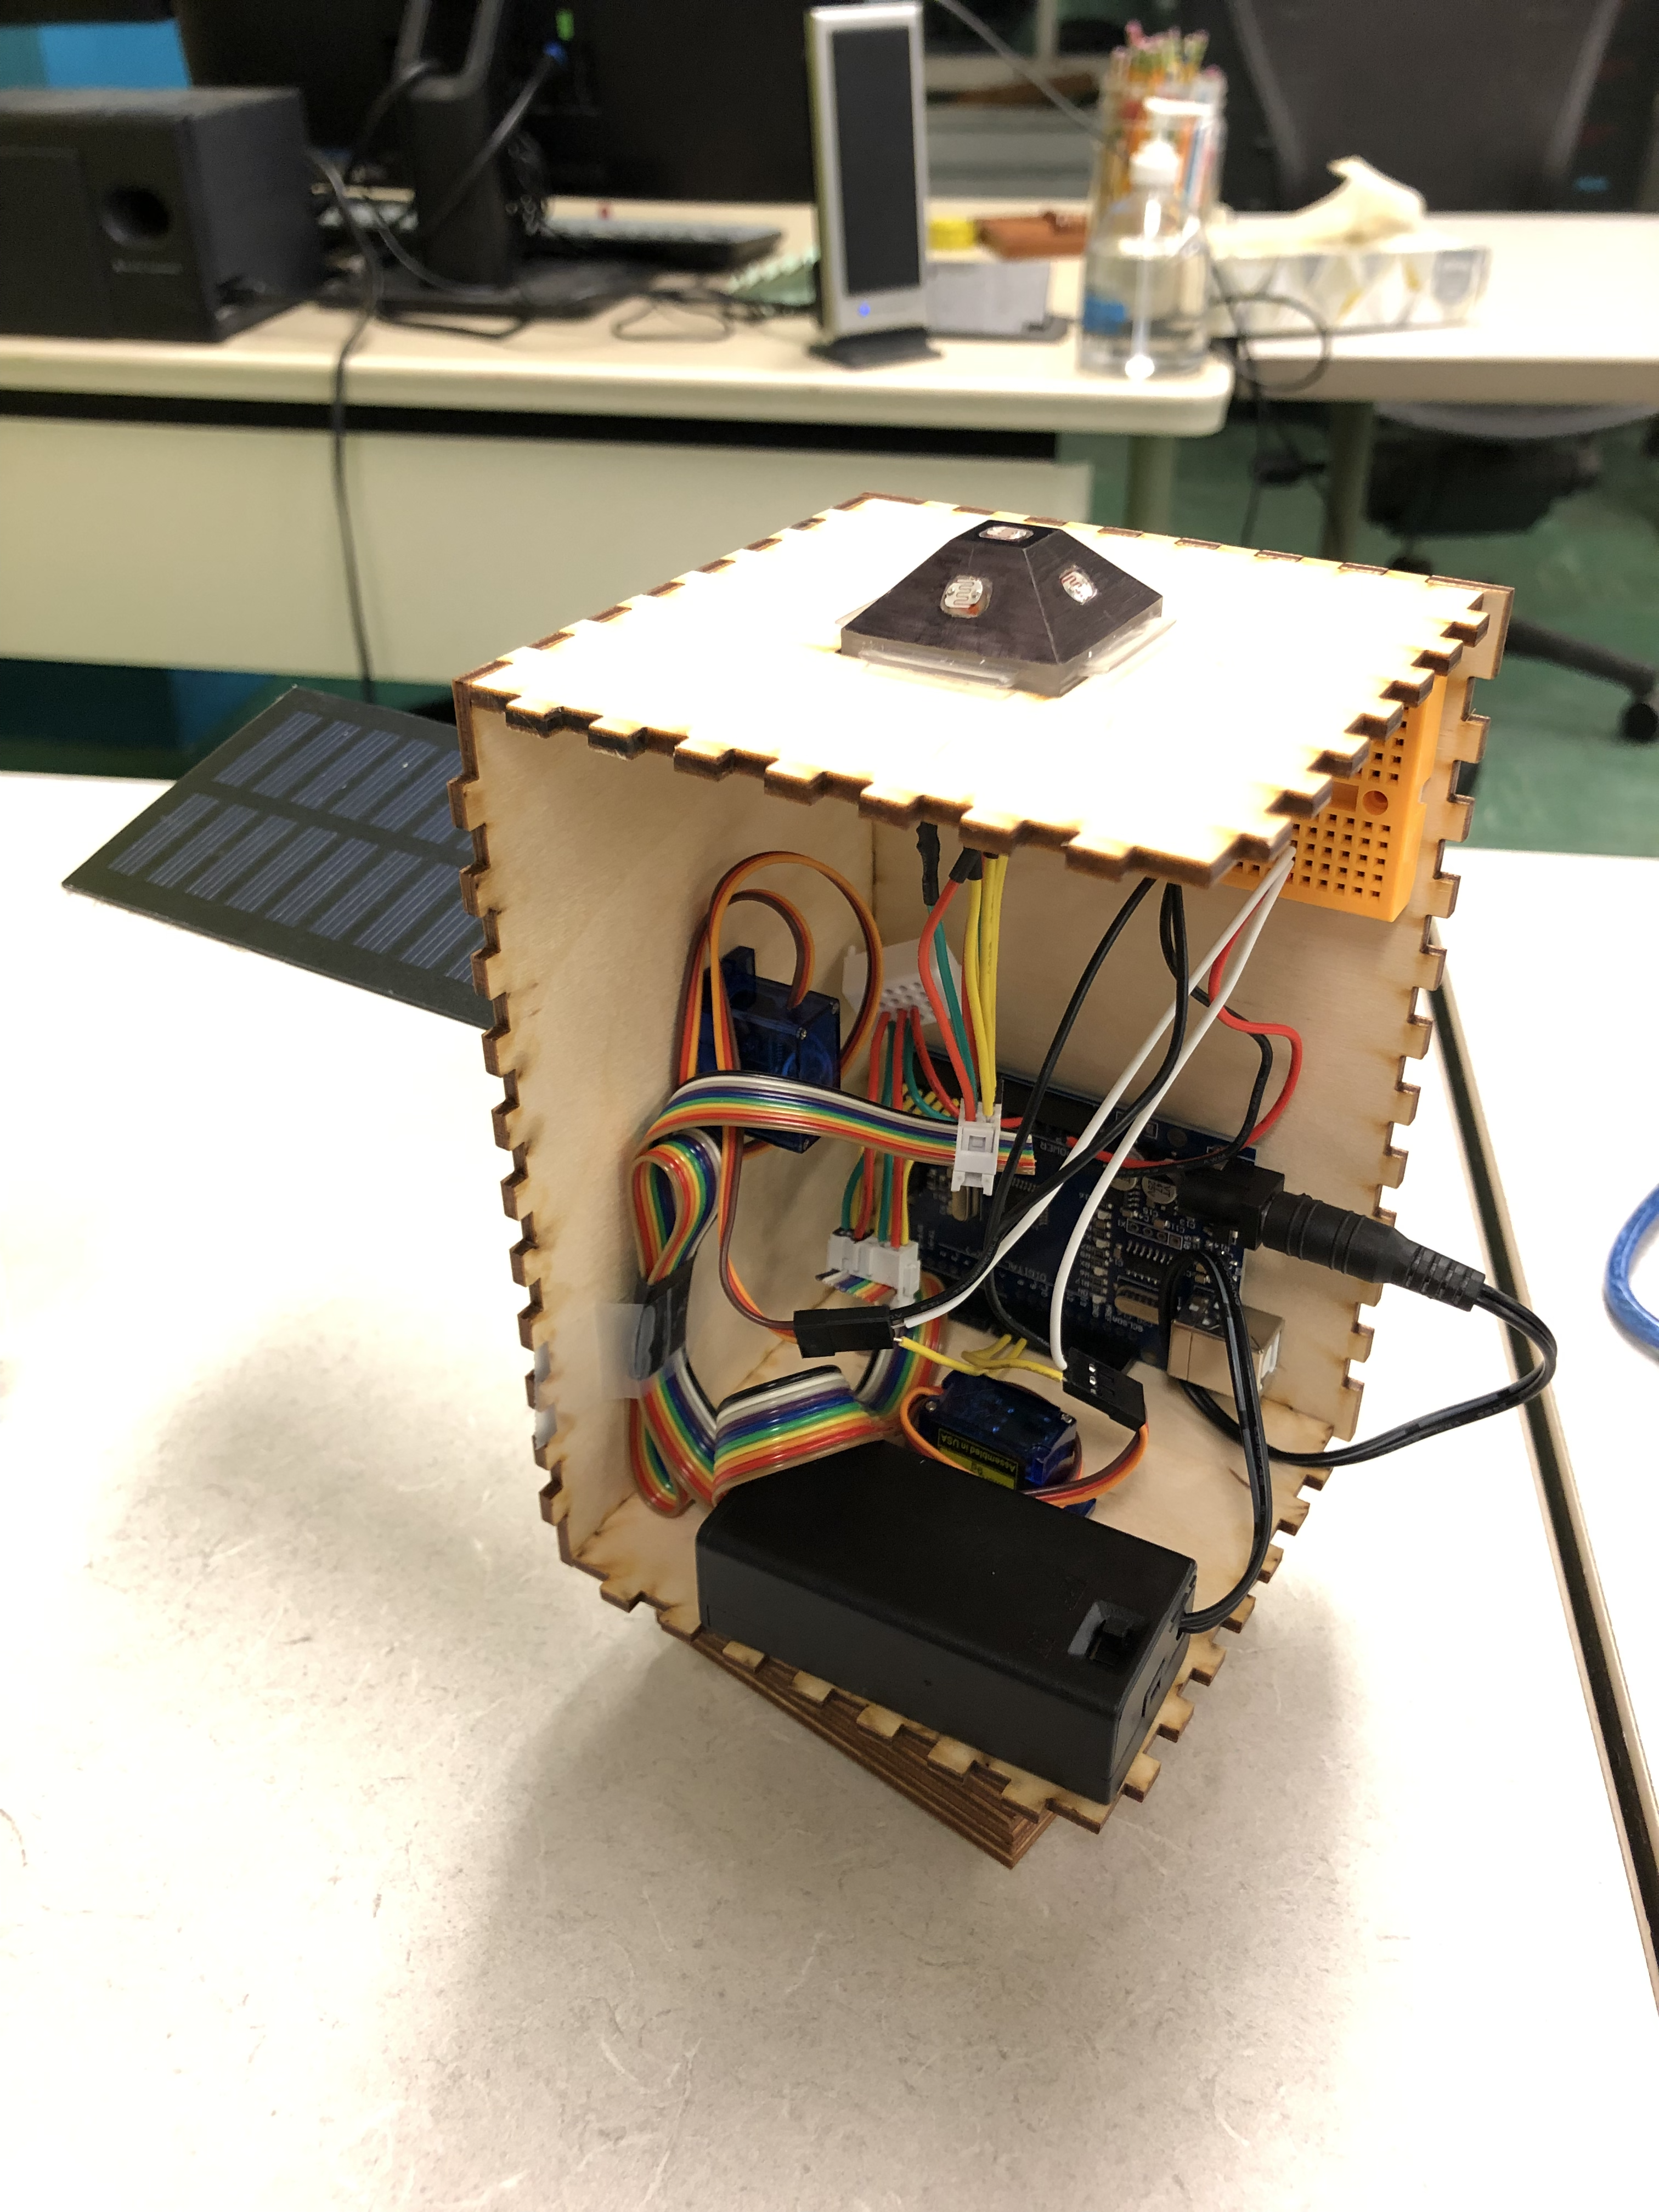
\includegraphics[width=0.55\linewidth, trim={0 0 0 0}, clip]{figures/satellite-completed.png}
    \caption{Completed mock satellite with internals shown.}
    \label{fig:satellite-completed}
\end{figure}

Hundreds of satellites are launched every year into space to conduct scientific research, provide communications services, and more. Almost all satellites are solar-powered, and those satellites must be able to point their solar panels toward the Sun. Unlike on Earth, there is no atmosphere in space to refract the sunlight, so precise pointing is required for the solar panels to receive the maximum amount of energy and power the satellite. 



\section{Sun Sensor Design}
\label{sec:sun-sensor}

The most challenging part of the project was the design and manufacturing of the sun sensor. A sun sensor measures the intensity of light from multiple angles and uses that information to calculate the direction of the sun. For my sun sensor design, I chose to use a truncated pyramid with sensors on each face excluding the bottom, which would give five different measurement directions. I planned to mount photoresistors on each face for light intensity detection. 

I created a sun sensor design in Fusion 360, shown in Figure~\ref{fig:sun-sensor-wireframe}. I wanted the sensor to be compact and robust --- since photoresistors are somewhat flimsy, I made slots on the faces for the photoresistors to fit into, along with channels for the leads.
\begin{figure}[!ht]
    \centering
    \includegraphics[width=0.8\linewidth]{figures/sun-sensor-wireframe.PNG}
    \caption{Wireframe view of the sun sensor design.}
    \label{fig:sun-sensor-wireframe}
\end{figure}

Since the design had many small details and hollow internals, I used resin printing instead of 3D printing. Surprisingly, the design worked on my first try. The resulting print with photoresistors is shown in Figure~\ref{fig:sun-sensor-pre-solder}. 

My design could have been improved in at least two ways. The four flanges coming out of each side of the sensor were printed without support, so the first few layers peeled off. The flanges are used to support the weight of the sun sensor when mounted in the satellite, so would have been better to make them more robust. 

Additionally, the channels inside the sun sensor were rather small, so there was a risk of the photoresistor leads touching each other, which would have shorted the sensor. I addressed this issue by adding small pieces of plywood between the leads to keep them separated. A better solution would have been to create separate channels for each of the positive and negative leads and reprint the sun sensor. 
\begin{figure}[!ht]
    \centering
    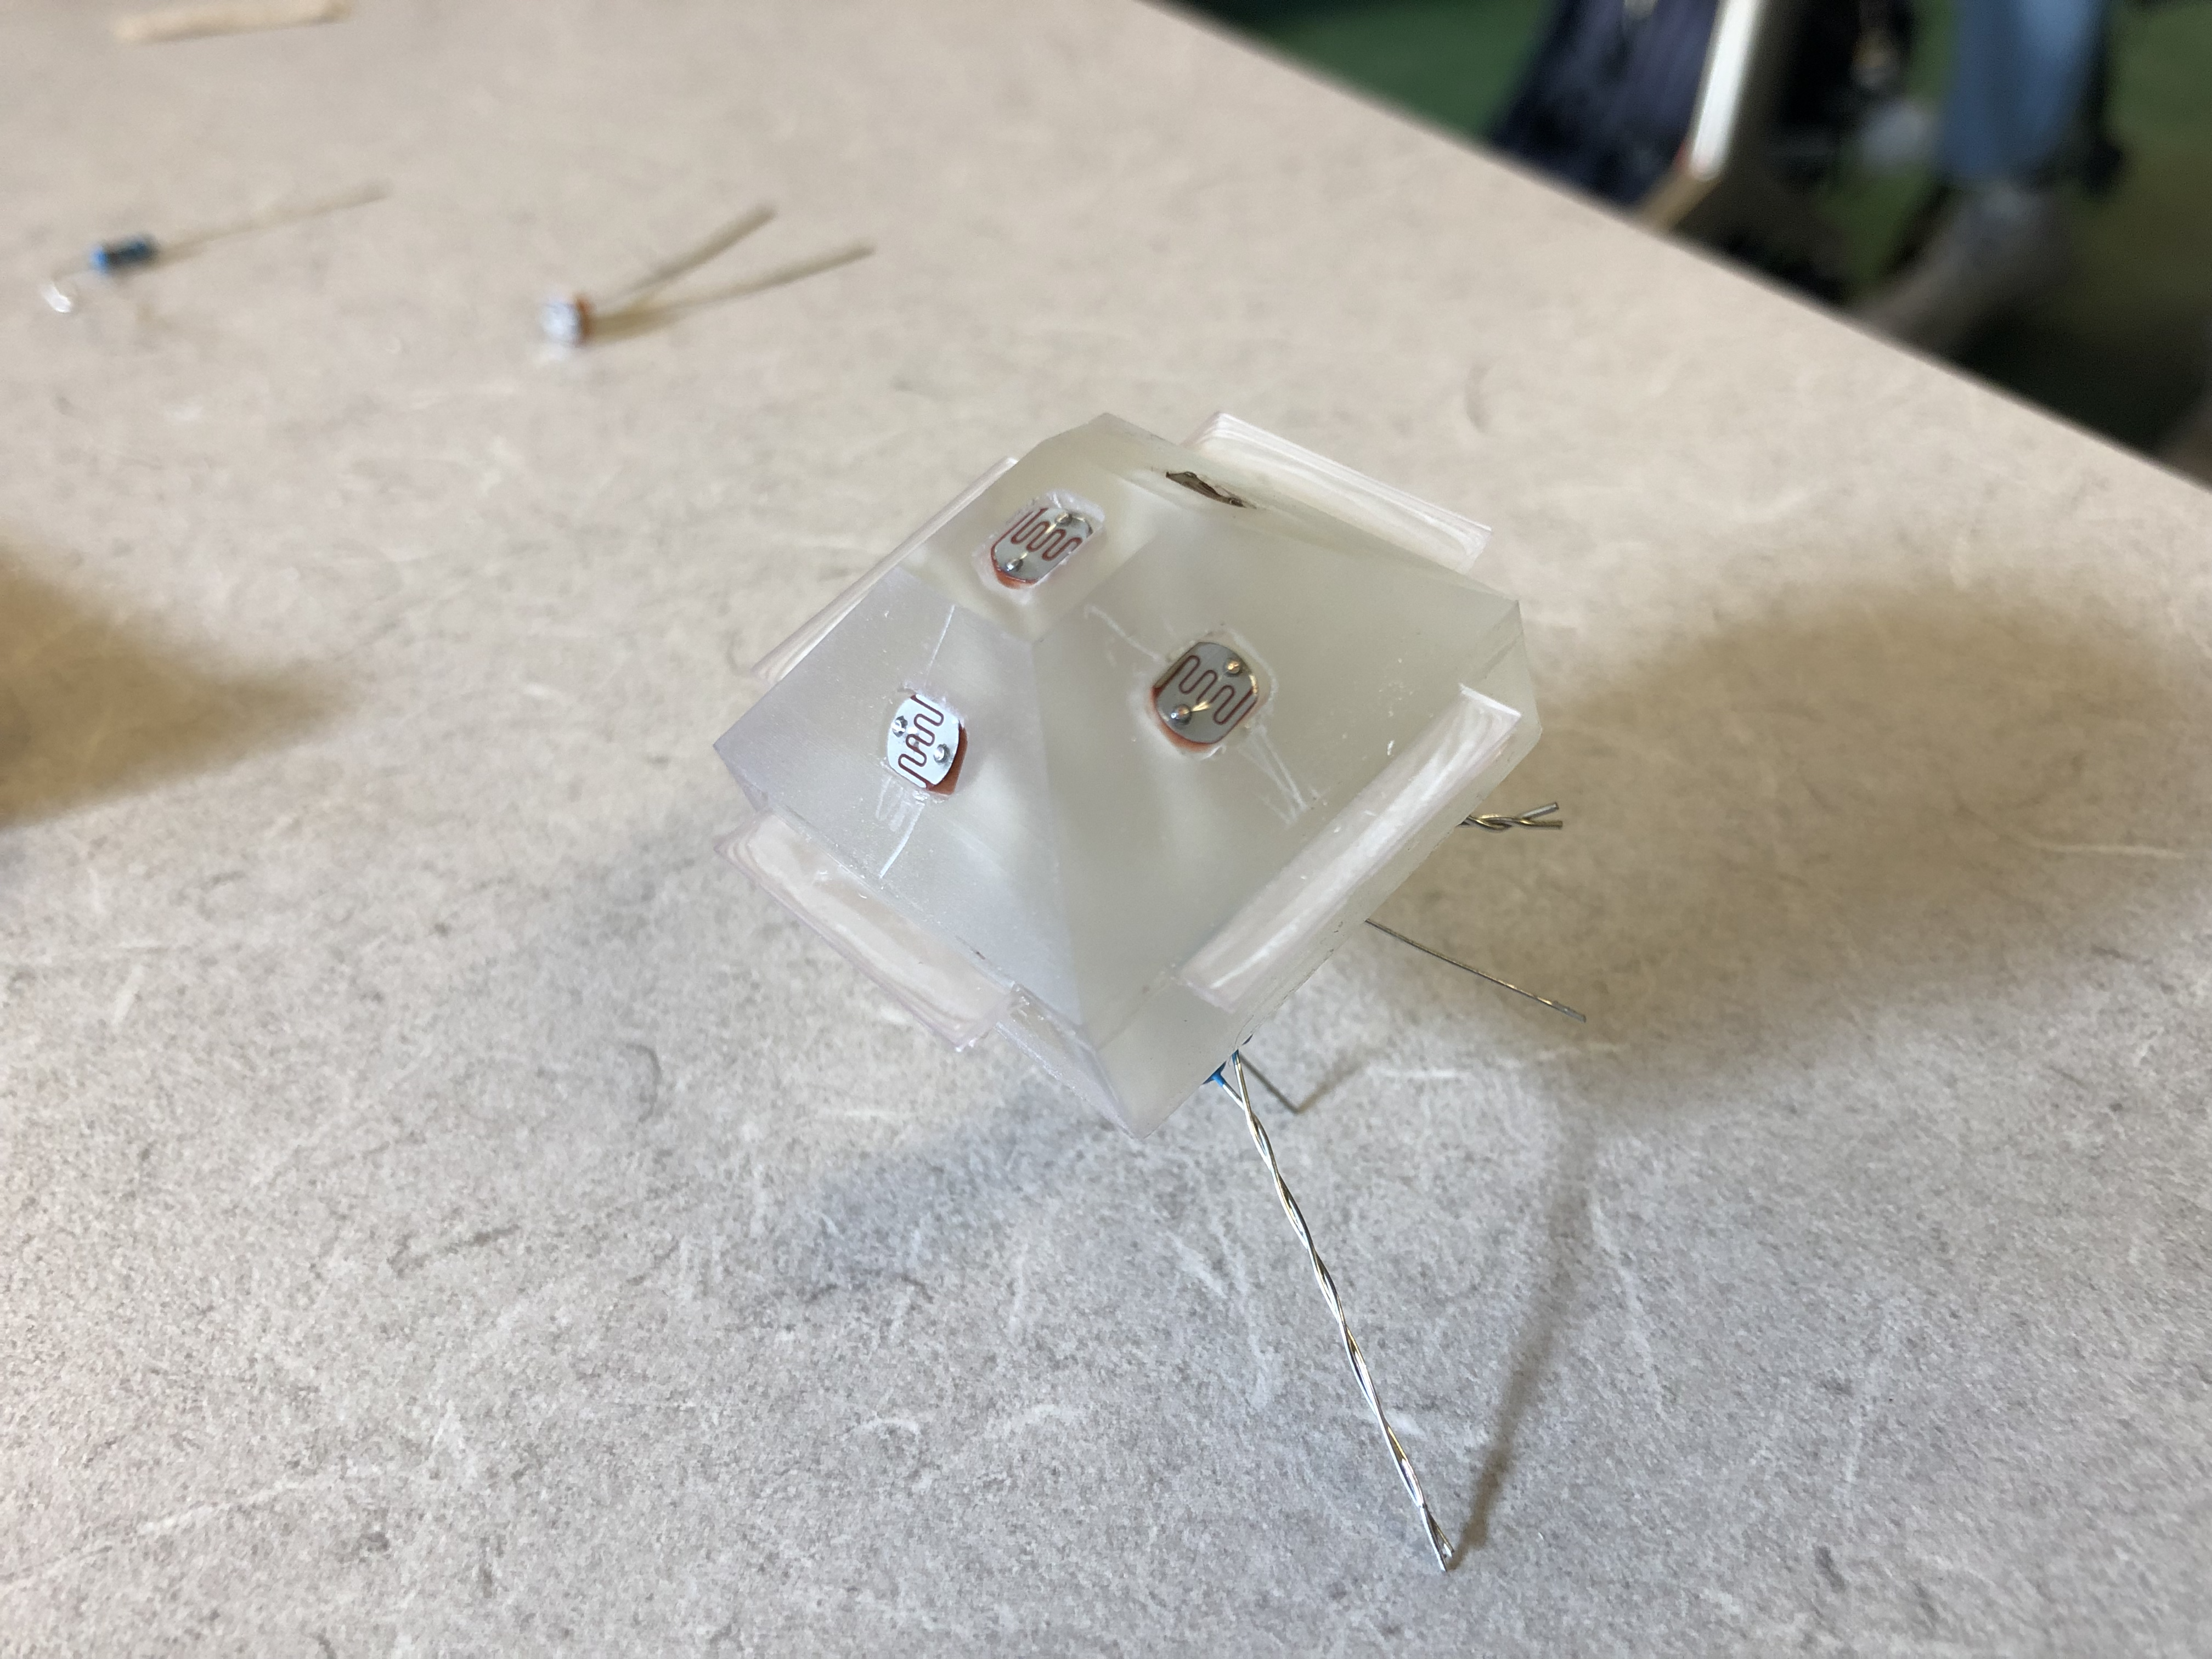
\includegraphics[width=0.8\linewidth]{figures/sun-sensor-pre-solder.png}
    \caption{Sun sensor resin print with photoresistors mounted.}
    \label{fig:sun-sensor-pre-solder}
\end{figure}

Next, I soldered resistors to each photoresistor, added heat-shrink tubing for insulation, and added a ribbon cable for easier interfacing with the Arduino. The result is shown in Figure~\ref{fig:sun-sensor-ribbon}. In hindsight, it would have been better to create a simple printed circuit board (PCB) to interface with the bottom of the sun sensor. This would have reduced the amount of soldering required and completely eliminated the need to braid wires together, making the design even more compact. 
\begin{figure}[!ht]
    \centering
    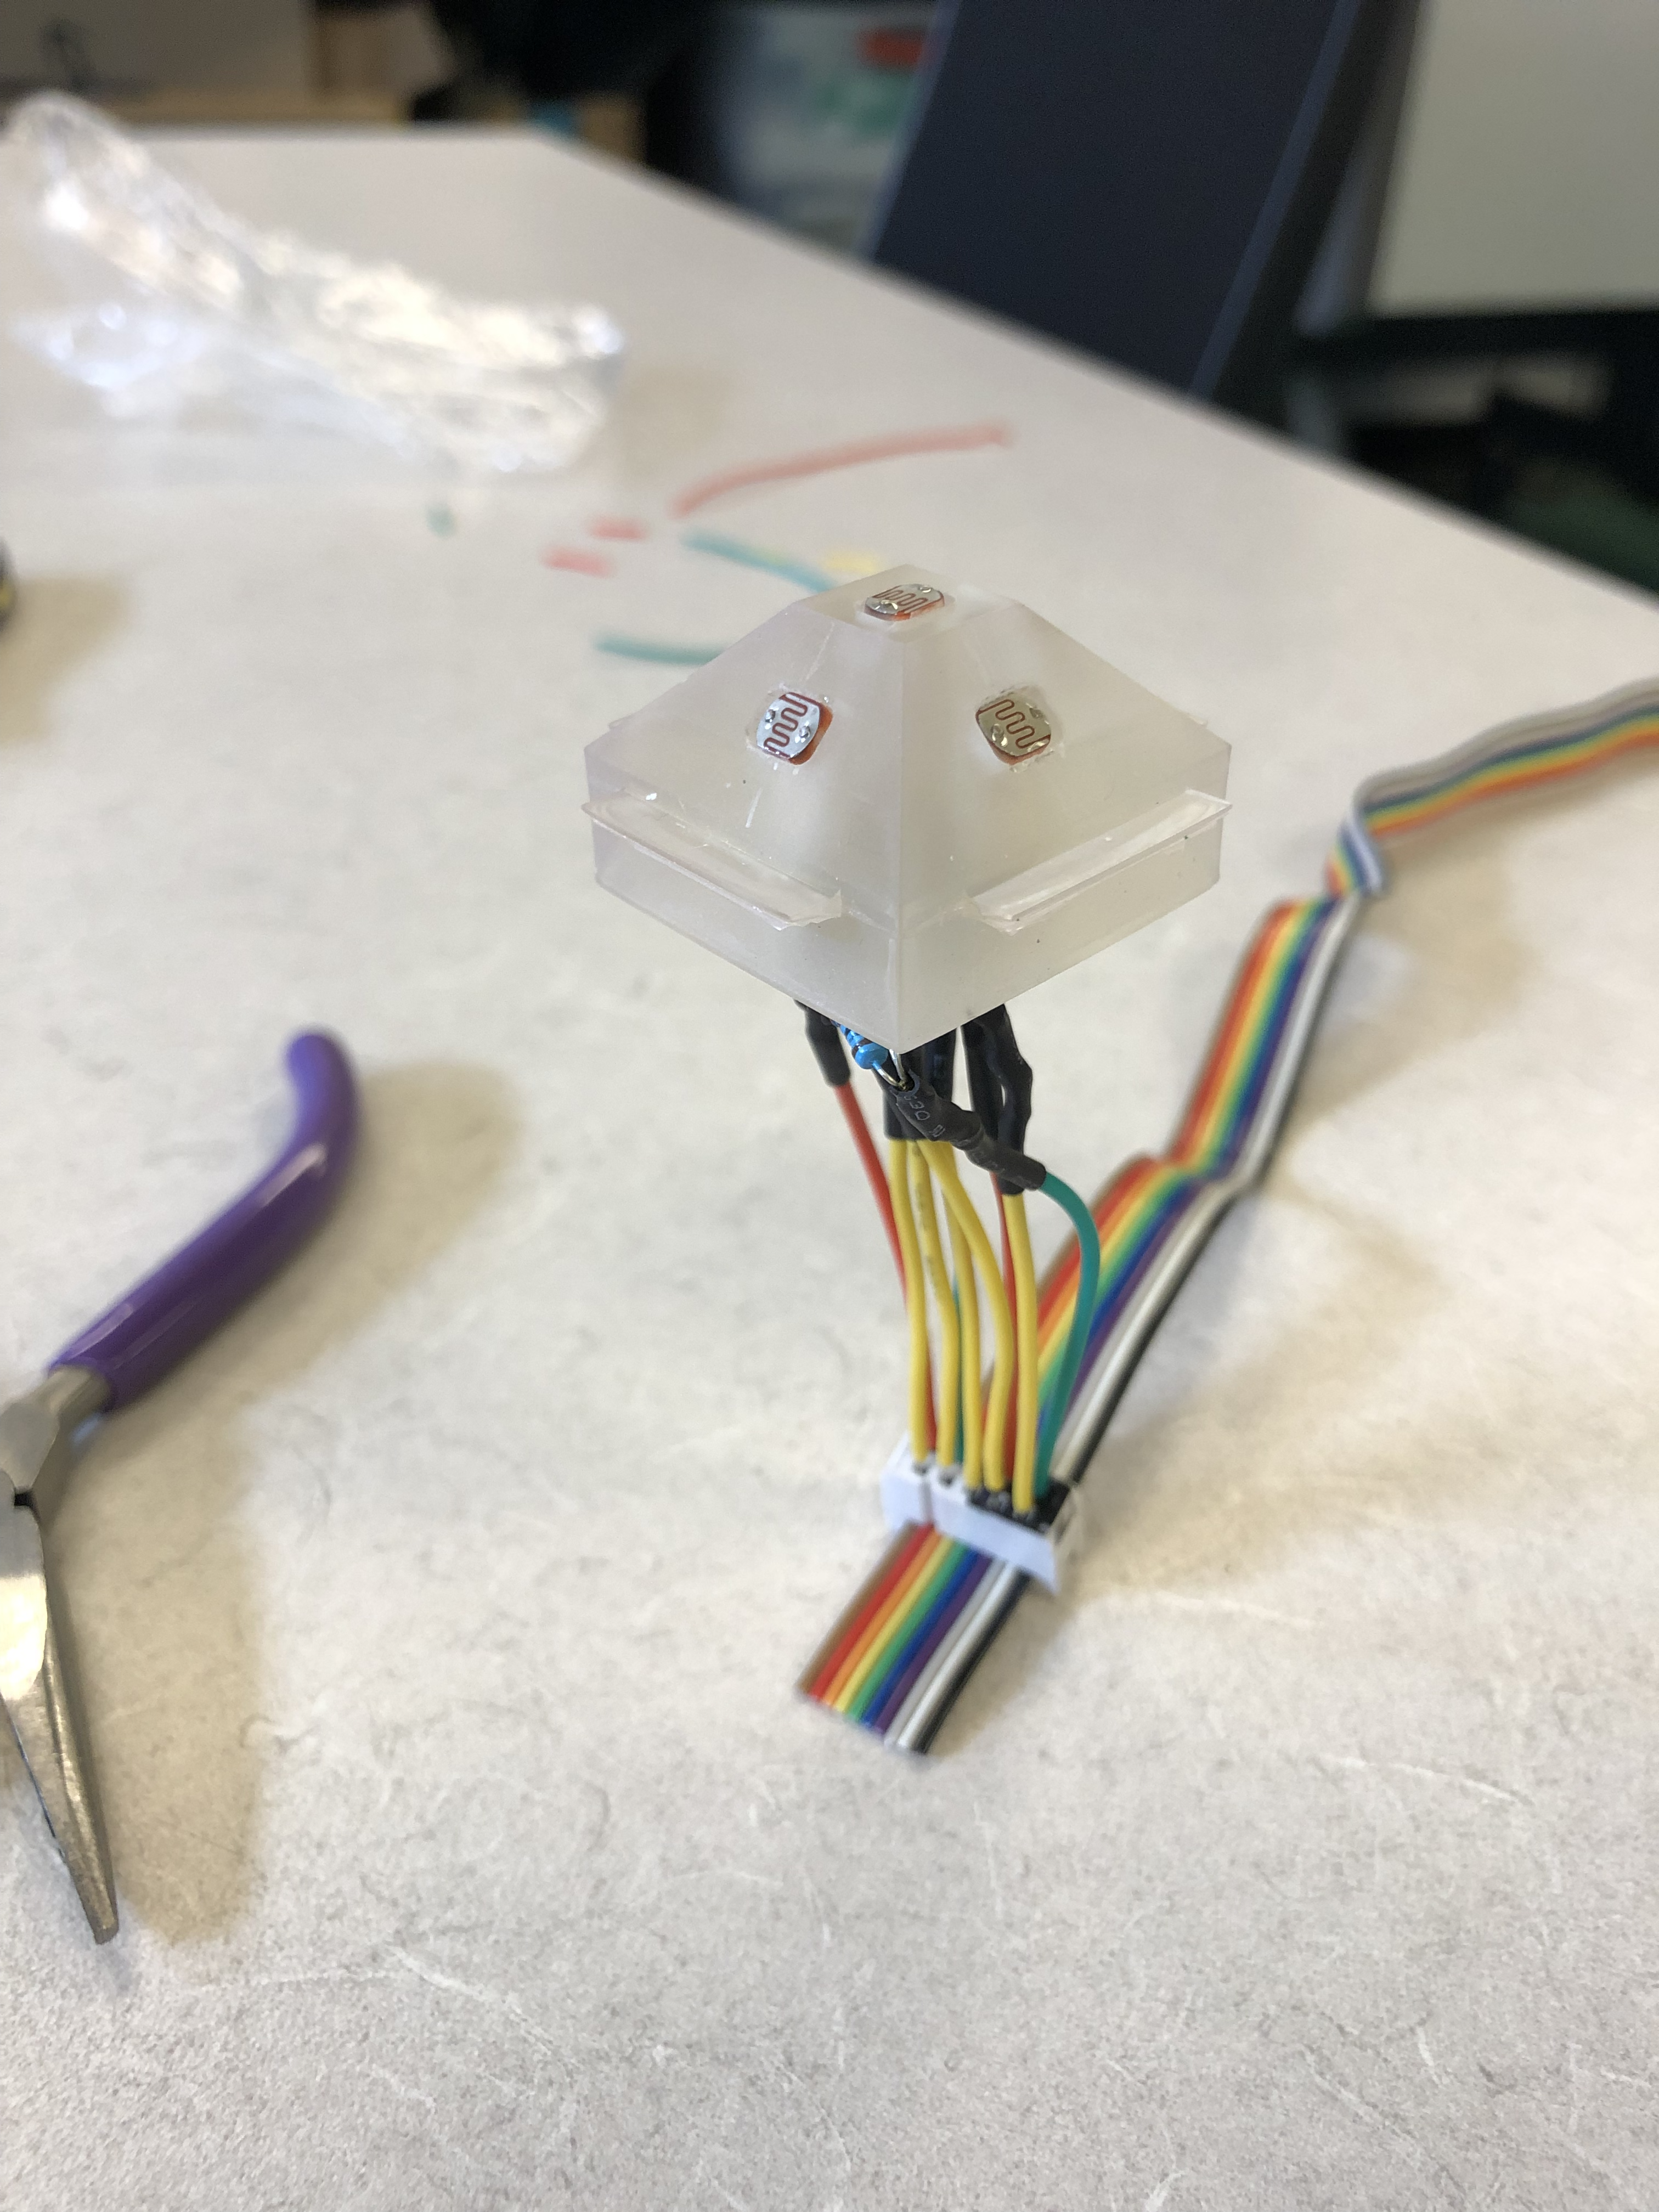
\includegraphics[width=0.55\linewidth]{figures/sun-sensor-ribbon.png}
    \caption{Completed sun sensor with ribbon cable attached.}
    \label{fig:sun-sensor-ribbon}
\end{figure}

Finally, I calibrated the sensors by measuring the output of each photoresistor while in near complete darkness and while under a bright flashlight, then wrote some Arduino code to test the functionality of the sun sensor. The finalized code is shown in Appendix~A.



\section{Build Highlights}
\label{sec:highlights}

The remainder of the build proceeded with very few issues, so only some highlights are covered here. The satellite is assembled from laser cut plywood with cutouts to for two servos and the sun sensor.

The mock satellite rotates on a stand via an SG90 servo. On my first attempt, I 3D printed an adapter for the servo arm, shown in Figure~\ref{fig:stand-3d-printed}. However, the servo had much more torque than I had anticipated and was far less rigid. Additionally, the stand had very little grip and was far lighter than the rest of the satellite. The combination fo these factors meant that the servo would cause the base to rotate more than the satellite itself, and the satellite would lean heavily to one side. 
\begin{figure}[!ht]
    \centering
    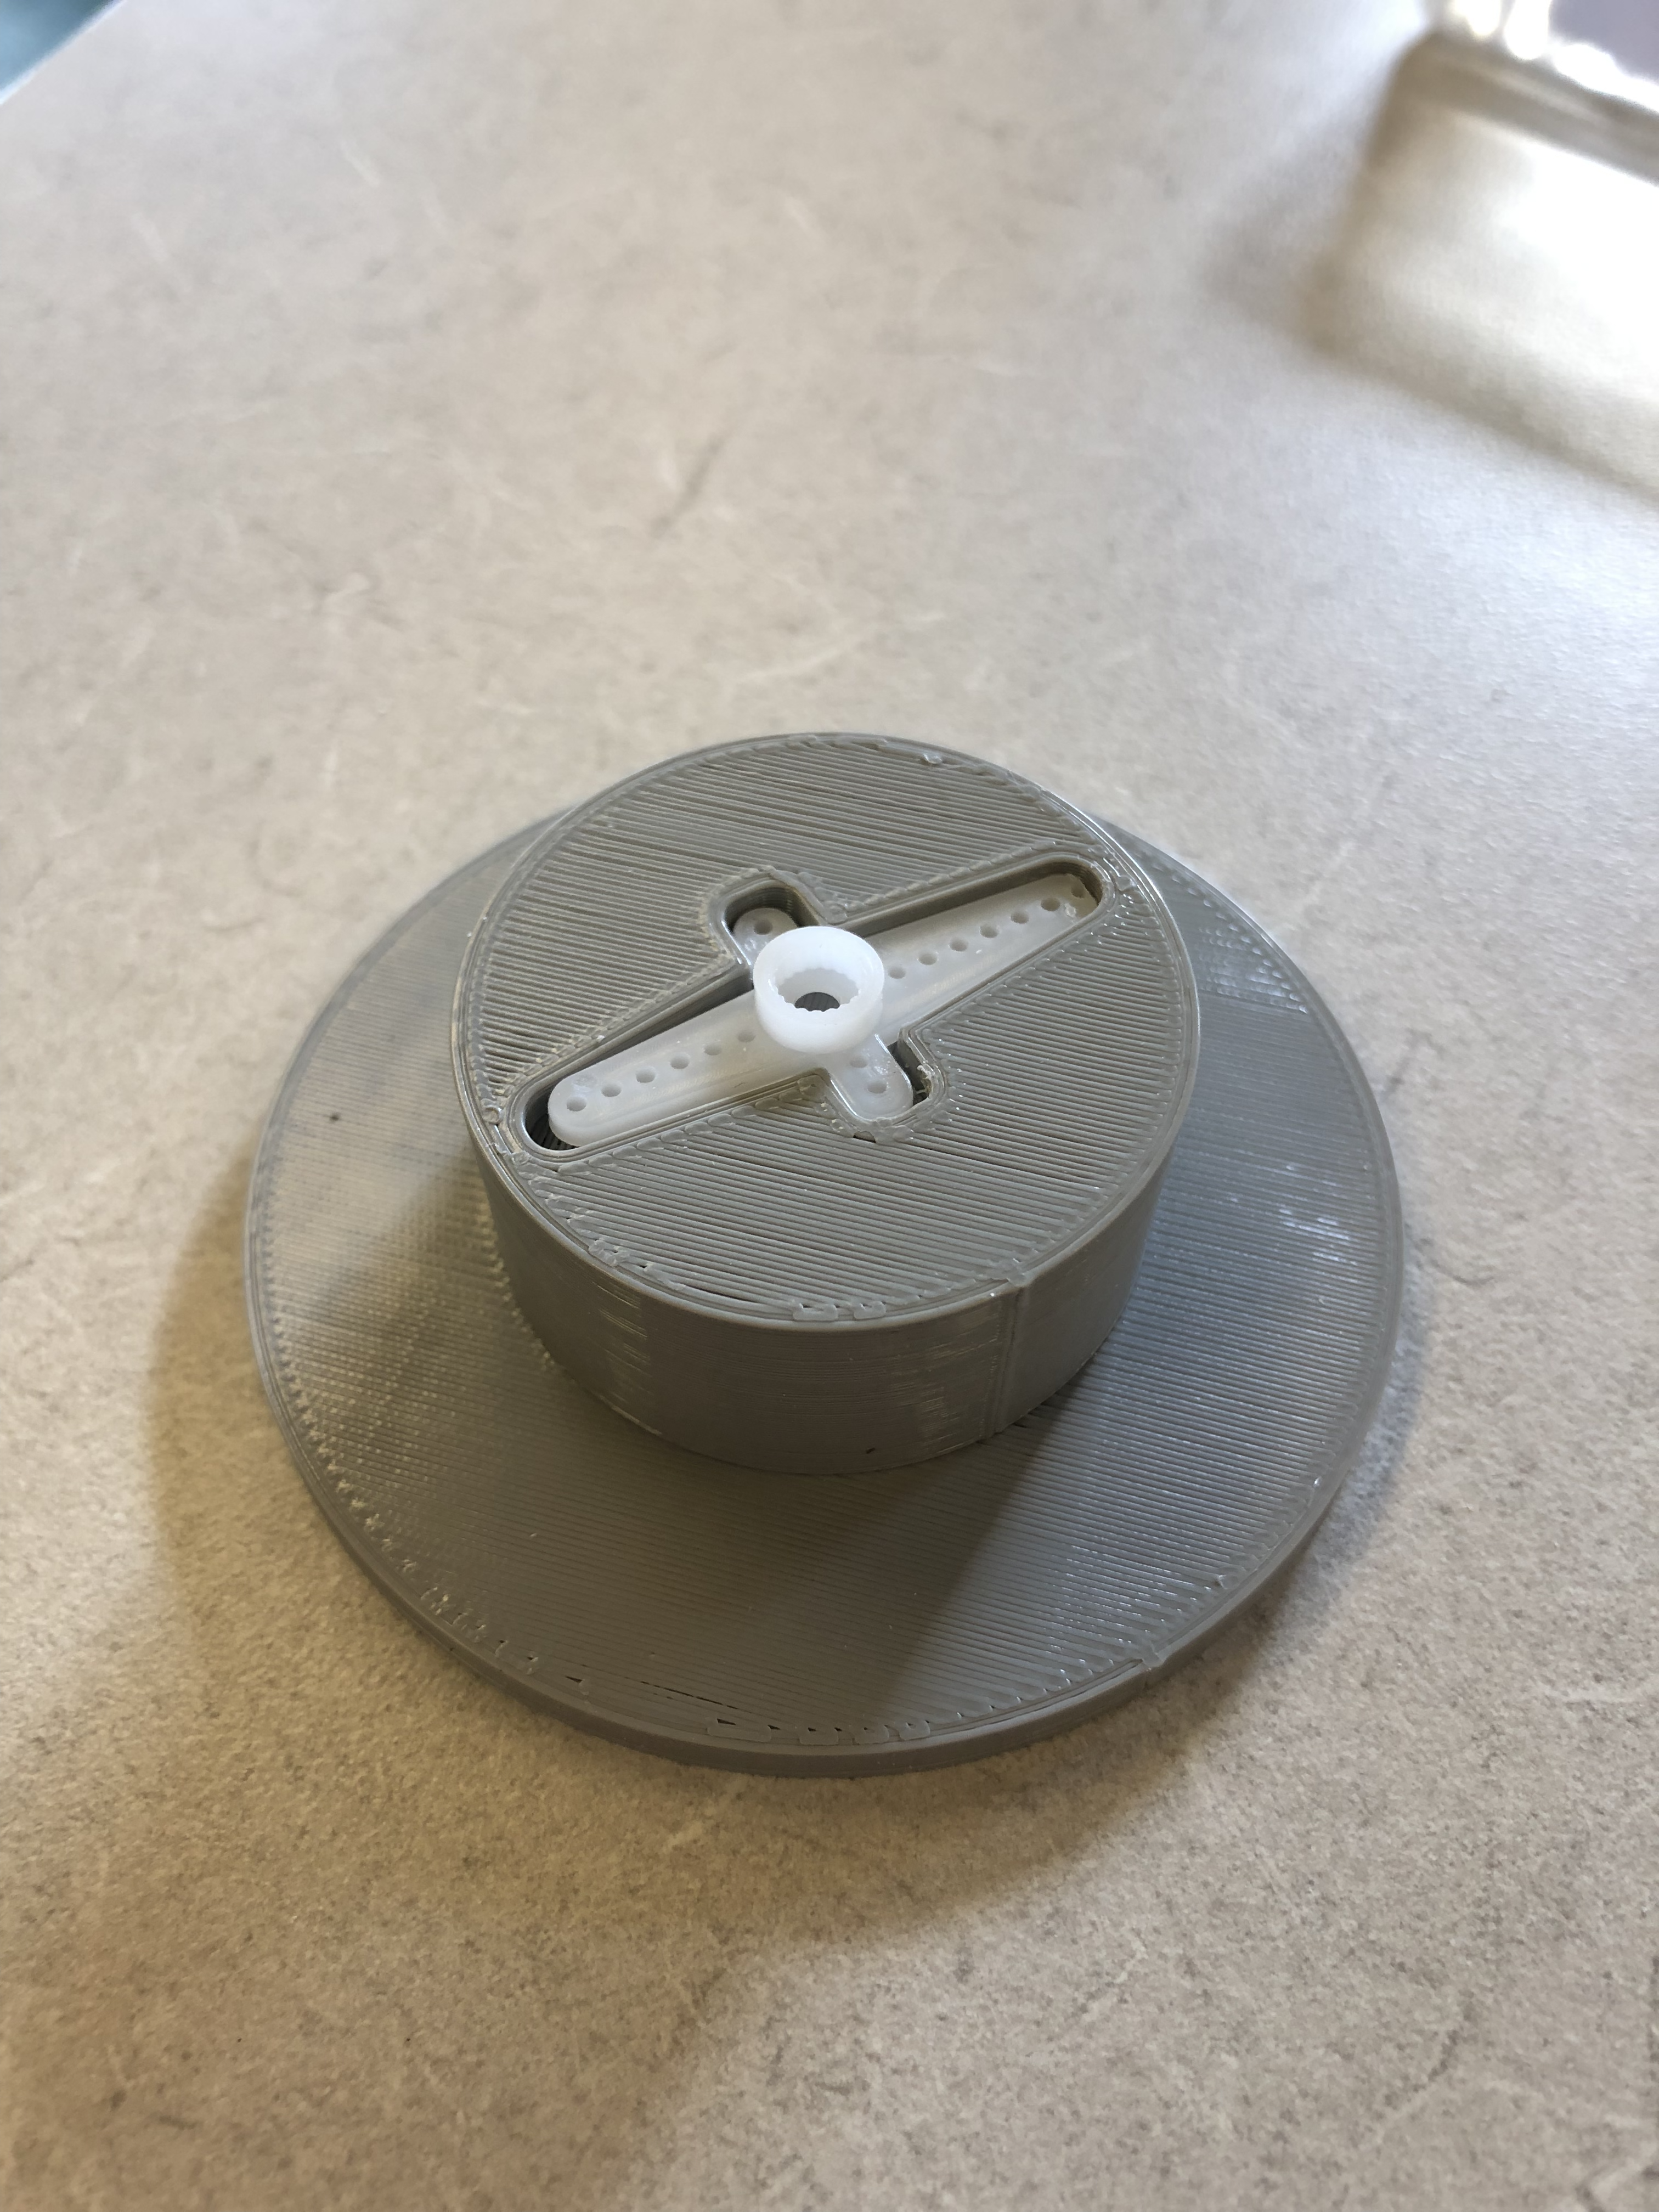
\includegraphics[width=0.6\linewidth, trim={0 200 0 700}, clip]{figures/stand-3d-printed.png}
    \caption{First iteration of 3D-printed satellite stand. }
    \label{fig:stand-3d-printed}
\end{figure}

I improved the design by laser cutting several plywood squares to fit over the existing stand. The plywood had holes to fit metal ball bearings so the satellite would by evenly supported. I also added rubber on the bottom to prevent slipping. The improved stand is shown in Figure~\ref{fig:base-with-bearing-detached}.
\begin{figure}[!ht]
    \centering
    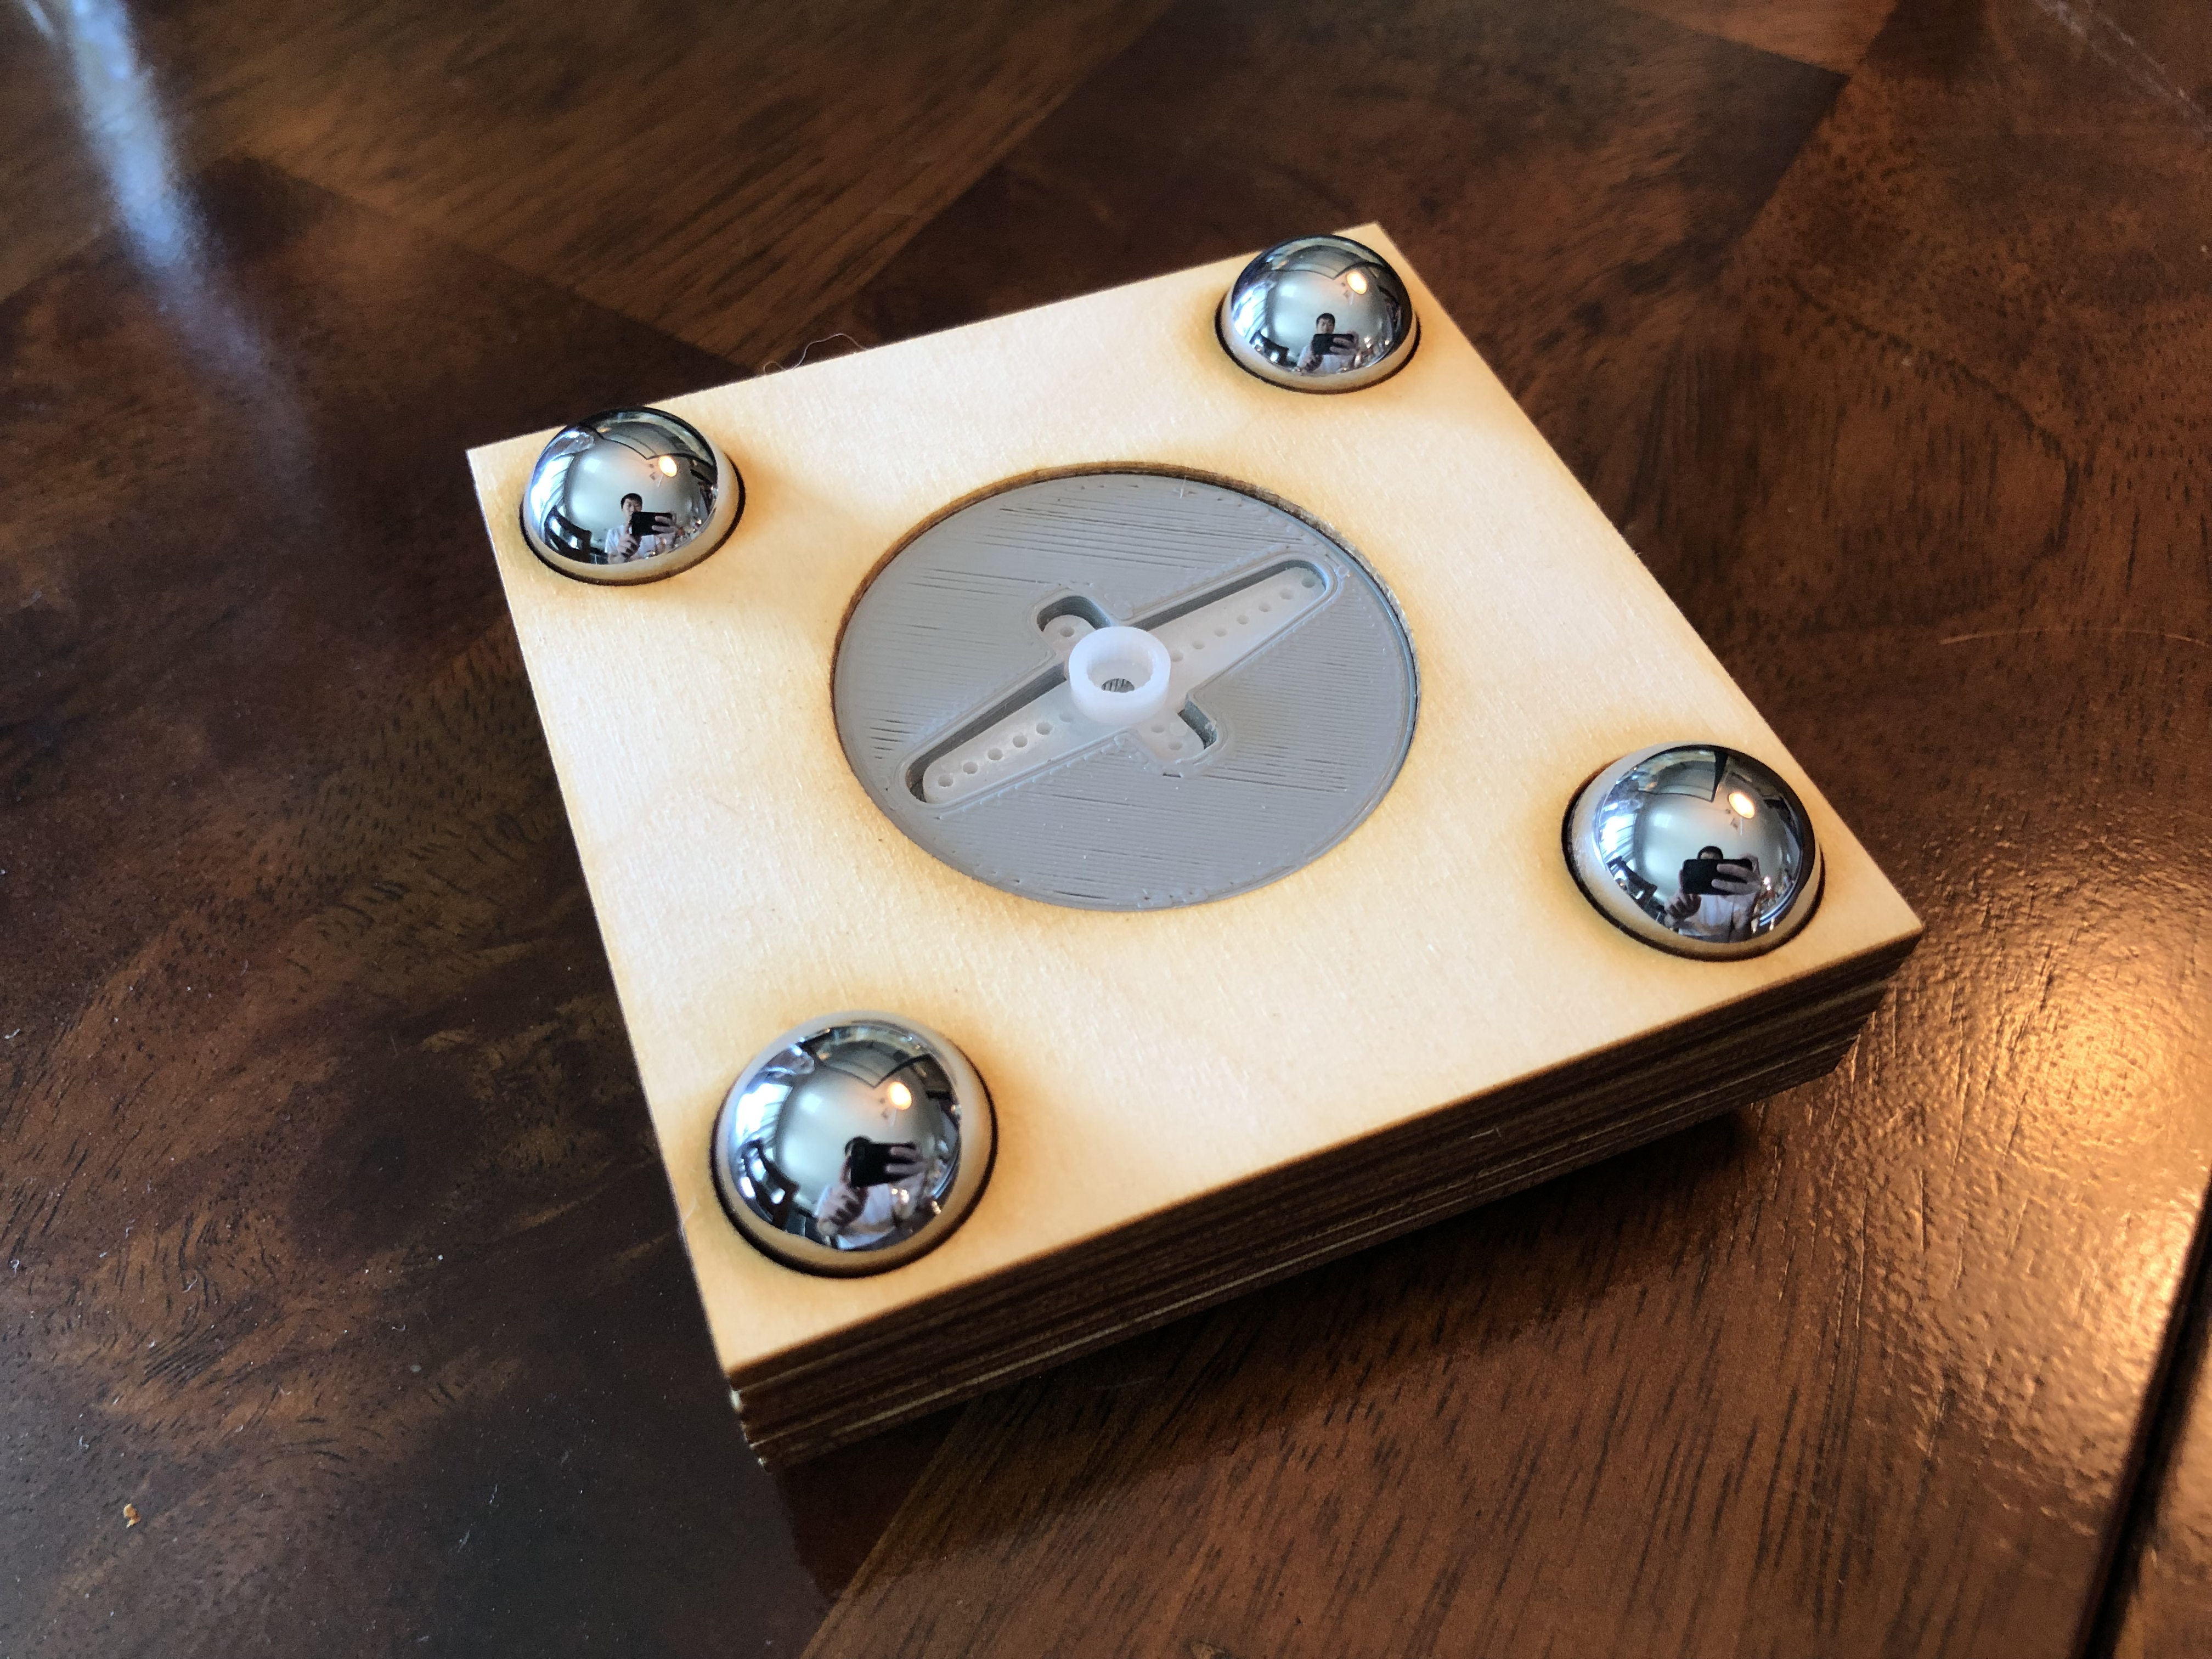
\includegraphics[width=0.8\linewidth]{figures/base-with-bearing-detached.png}
    \caption{Second iteration of the satellite stand with plywood and ball bearing support.}
    \label{fig:base-with-bearing-detached}
\end{figure}

The solar panel is mounted onto the side of the satellite and rotates using another SG90 servo. The supports were designed in Inkspace and laser cut from plywood, with the end result shown in Figure~\ref{fig:solar-panel-support}.
\begin{figure}[!ht]
	\centering
	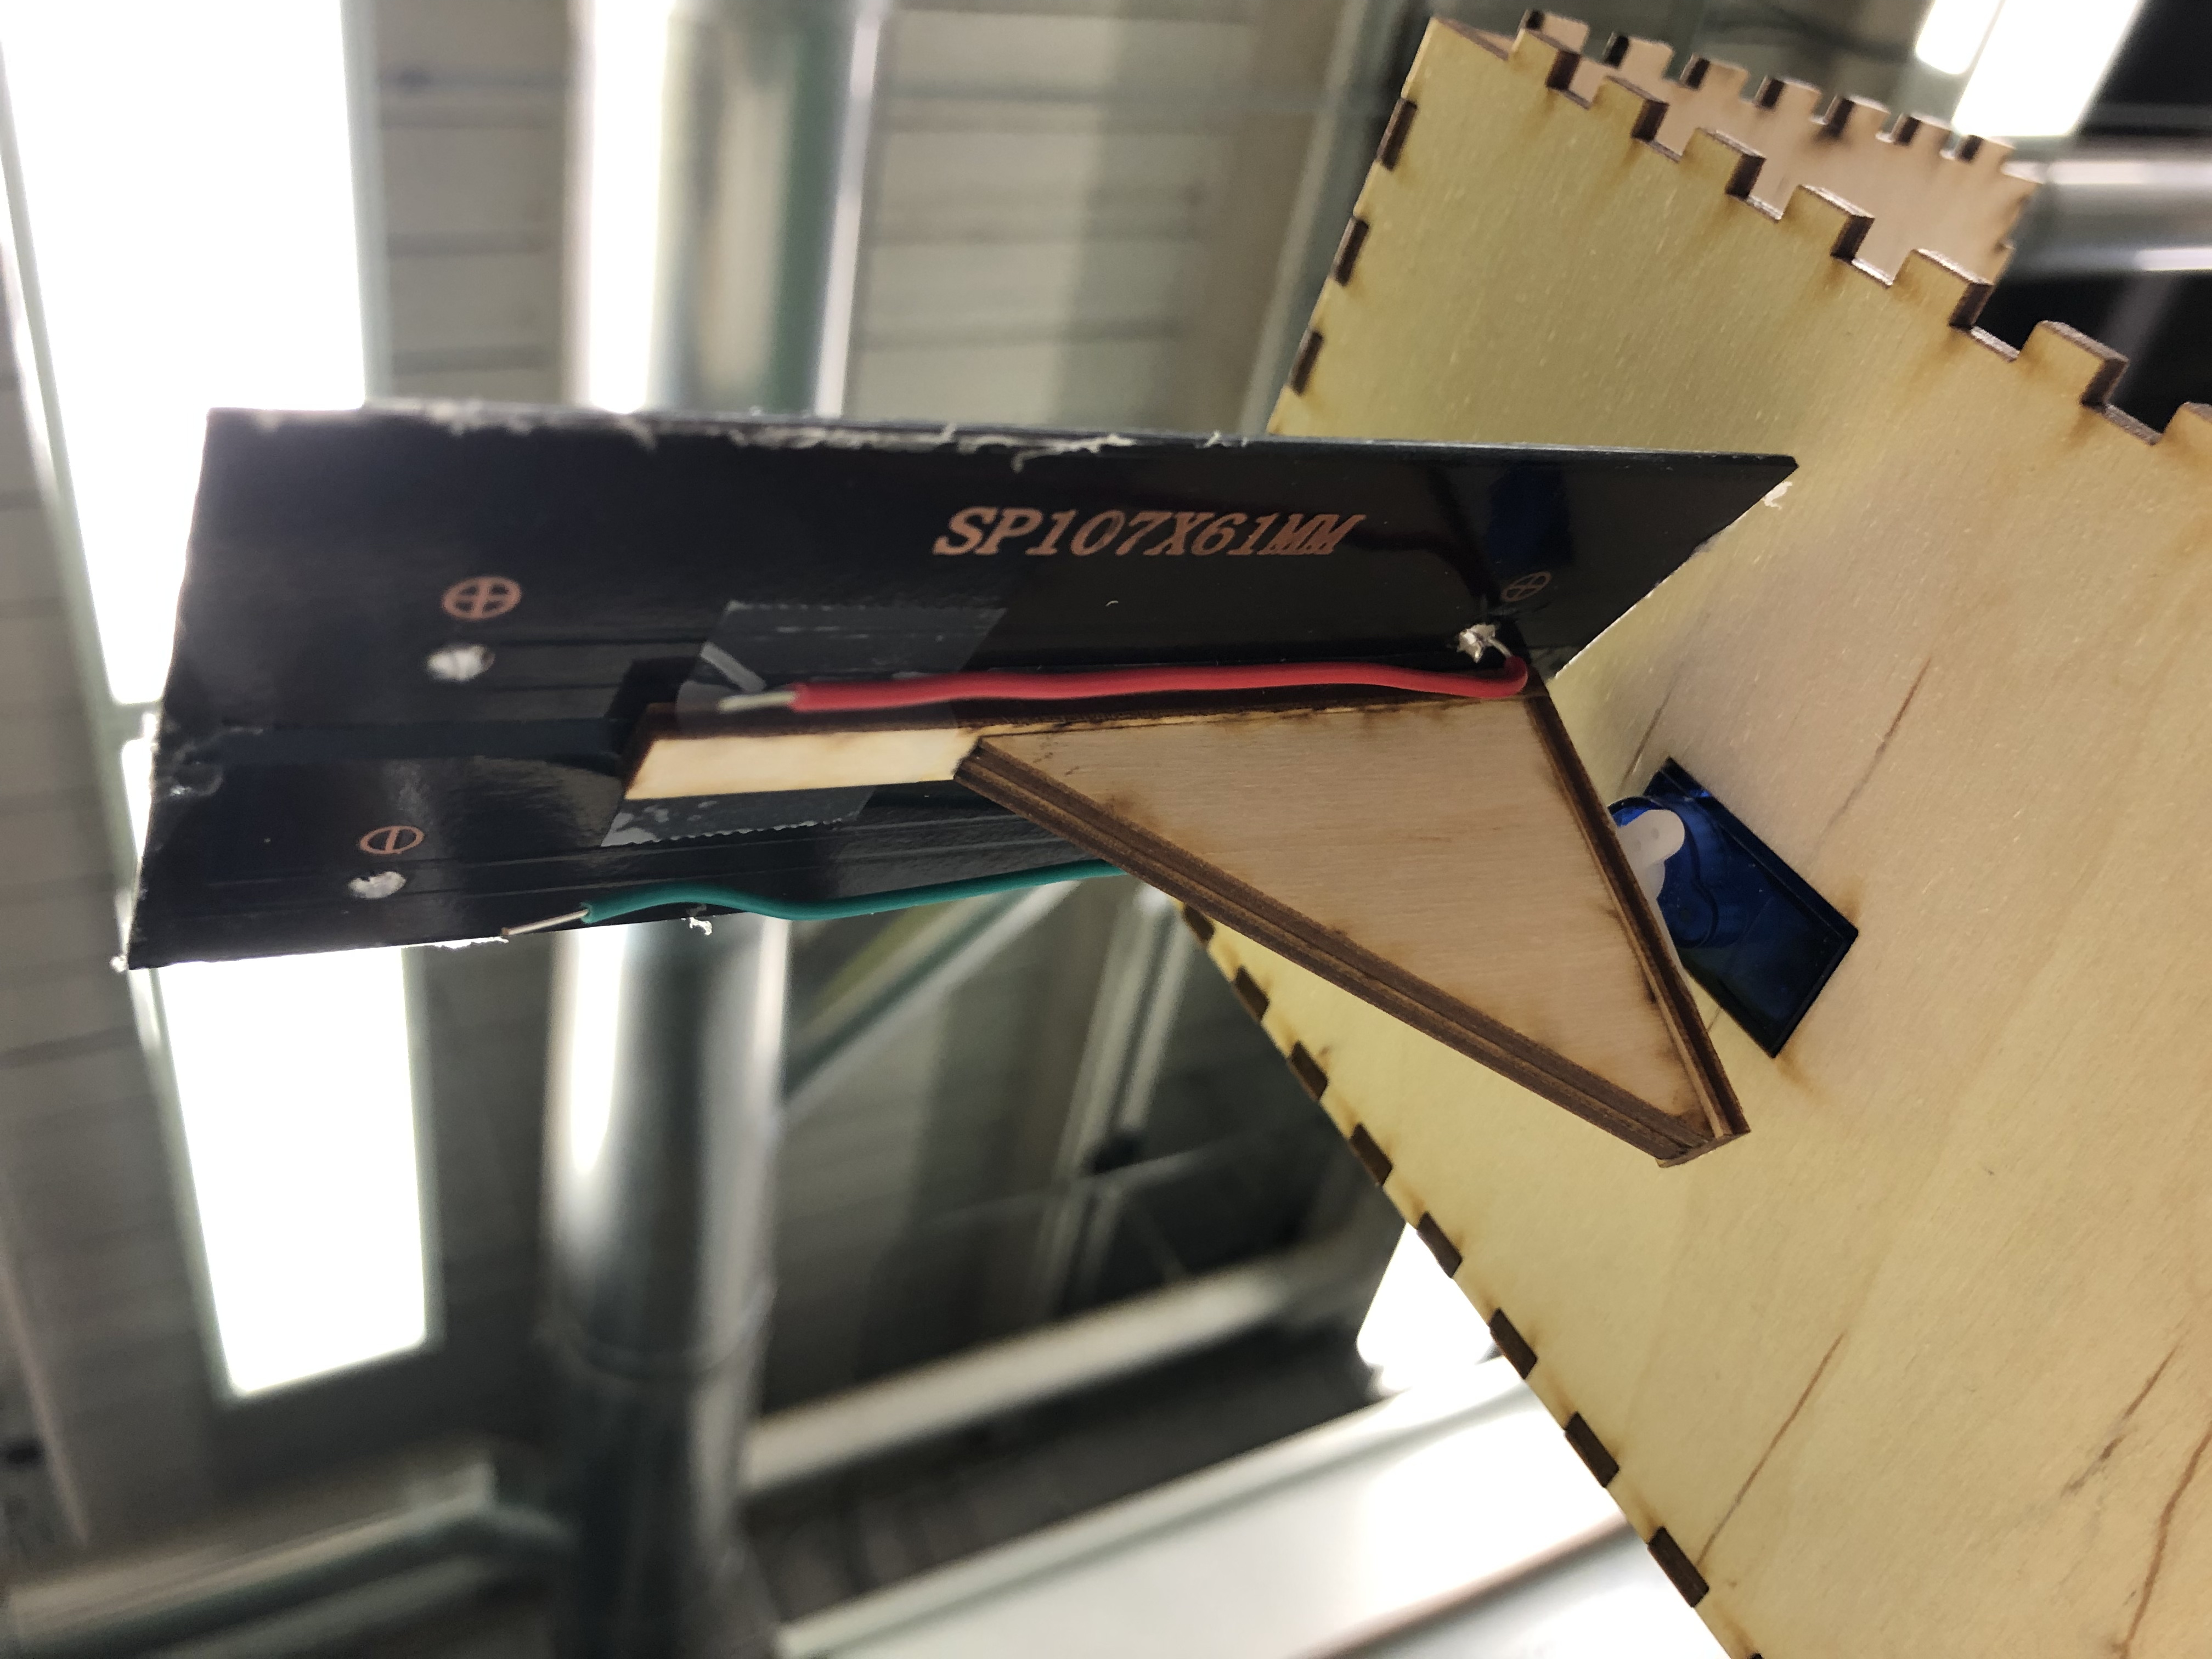
\includegraphics[width=0.8\linewidth]{figures/solar-panel-support.png}
	\caption{Solar panel mounted on the side of the satellite.}
	\label{fig:solar-panel-support}
\end{figure}




\FloatBarrier
\section{Testing and Demo}
\label{sec:testing}

Testing was done in two parts. As mentioned previously, the sun sensor was tested by itself after being assembled. I wrote some Arduino code to compute and display the direction of the light source based on the signal strength from each photoresistor (recall from an earlier section that their signal strengths were calibrated). I used a flashlight to test the performance of the sun sensor at different angles. 

I did not realize that the resin used to print the sun sensor would be translucent, which led to some problems with the photoresistor detecting light being refracted from the opposite direction that it was facing. This was resolved by simply coloring the exposed sides of the sun sensor with a black marker as shown in Figure~\ref{fig:sun-sensor-painted}. 
\begin{figure}[!ht]
	\centering
	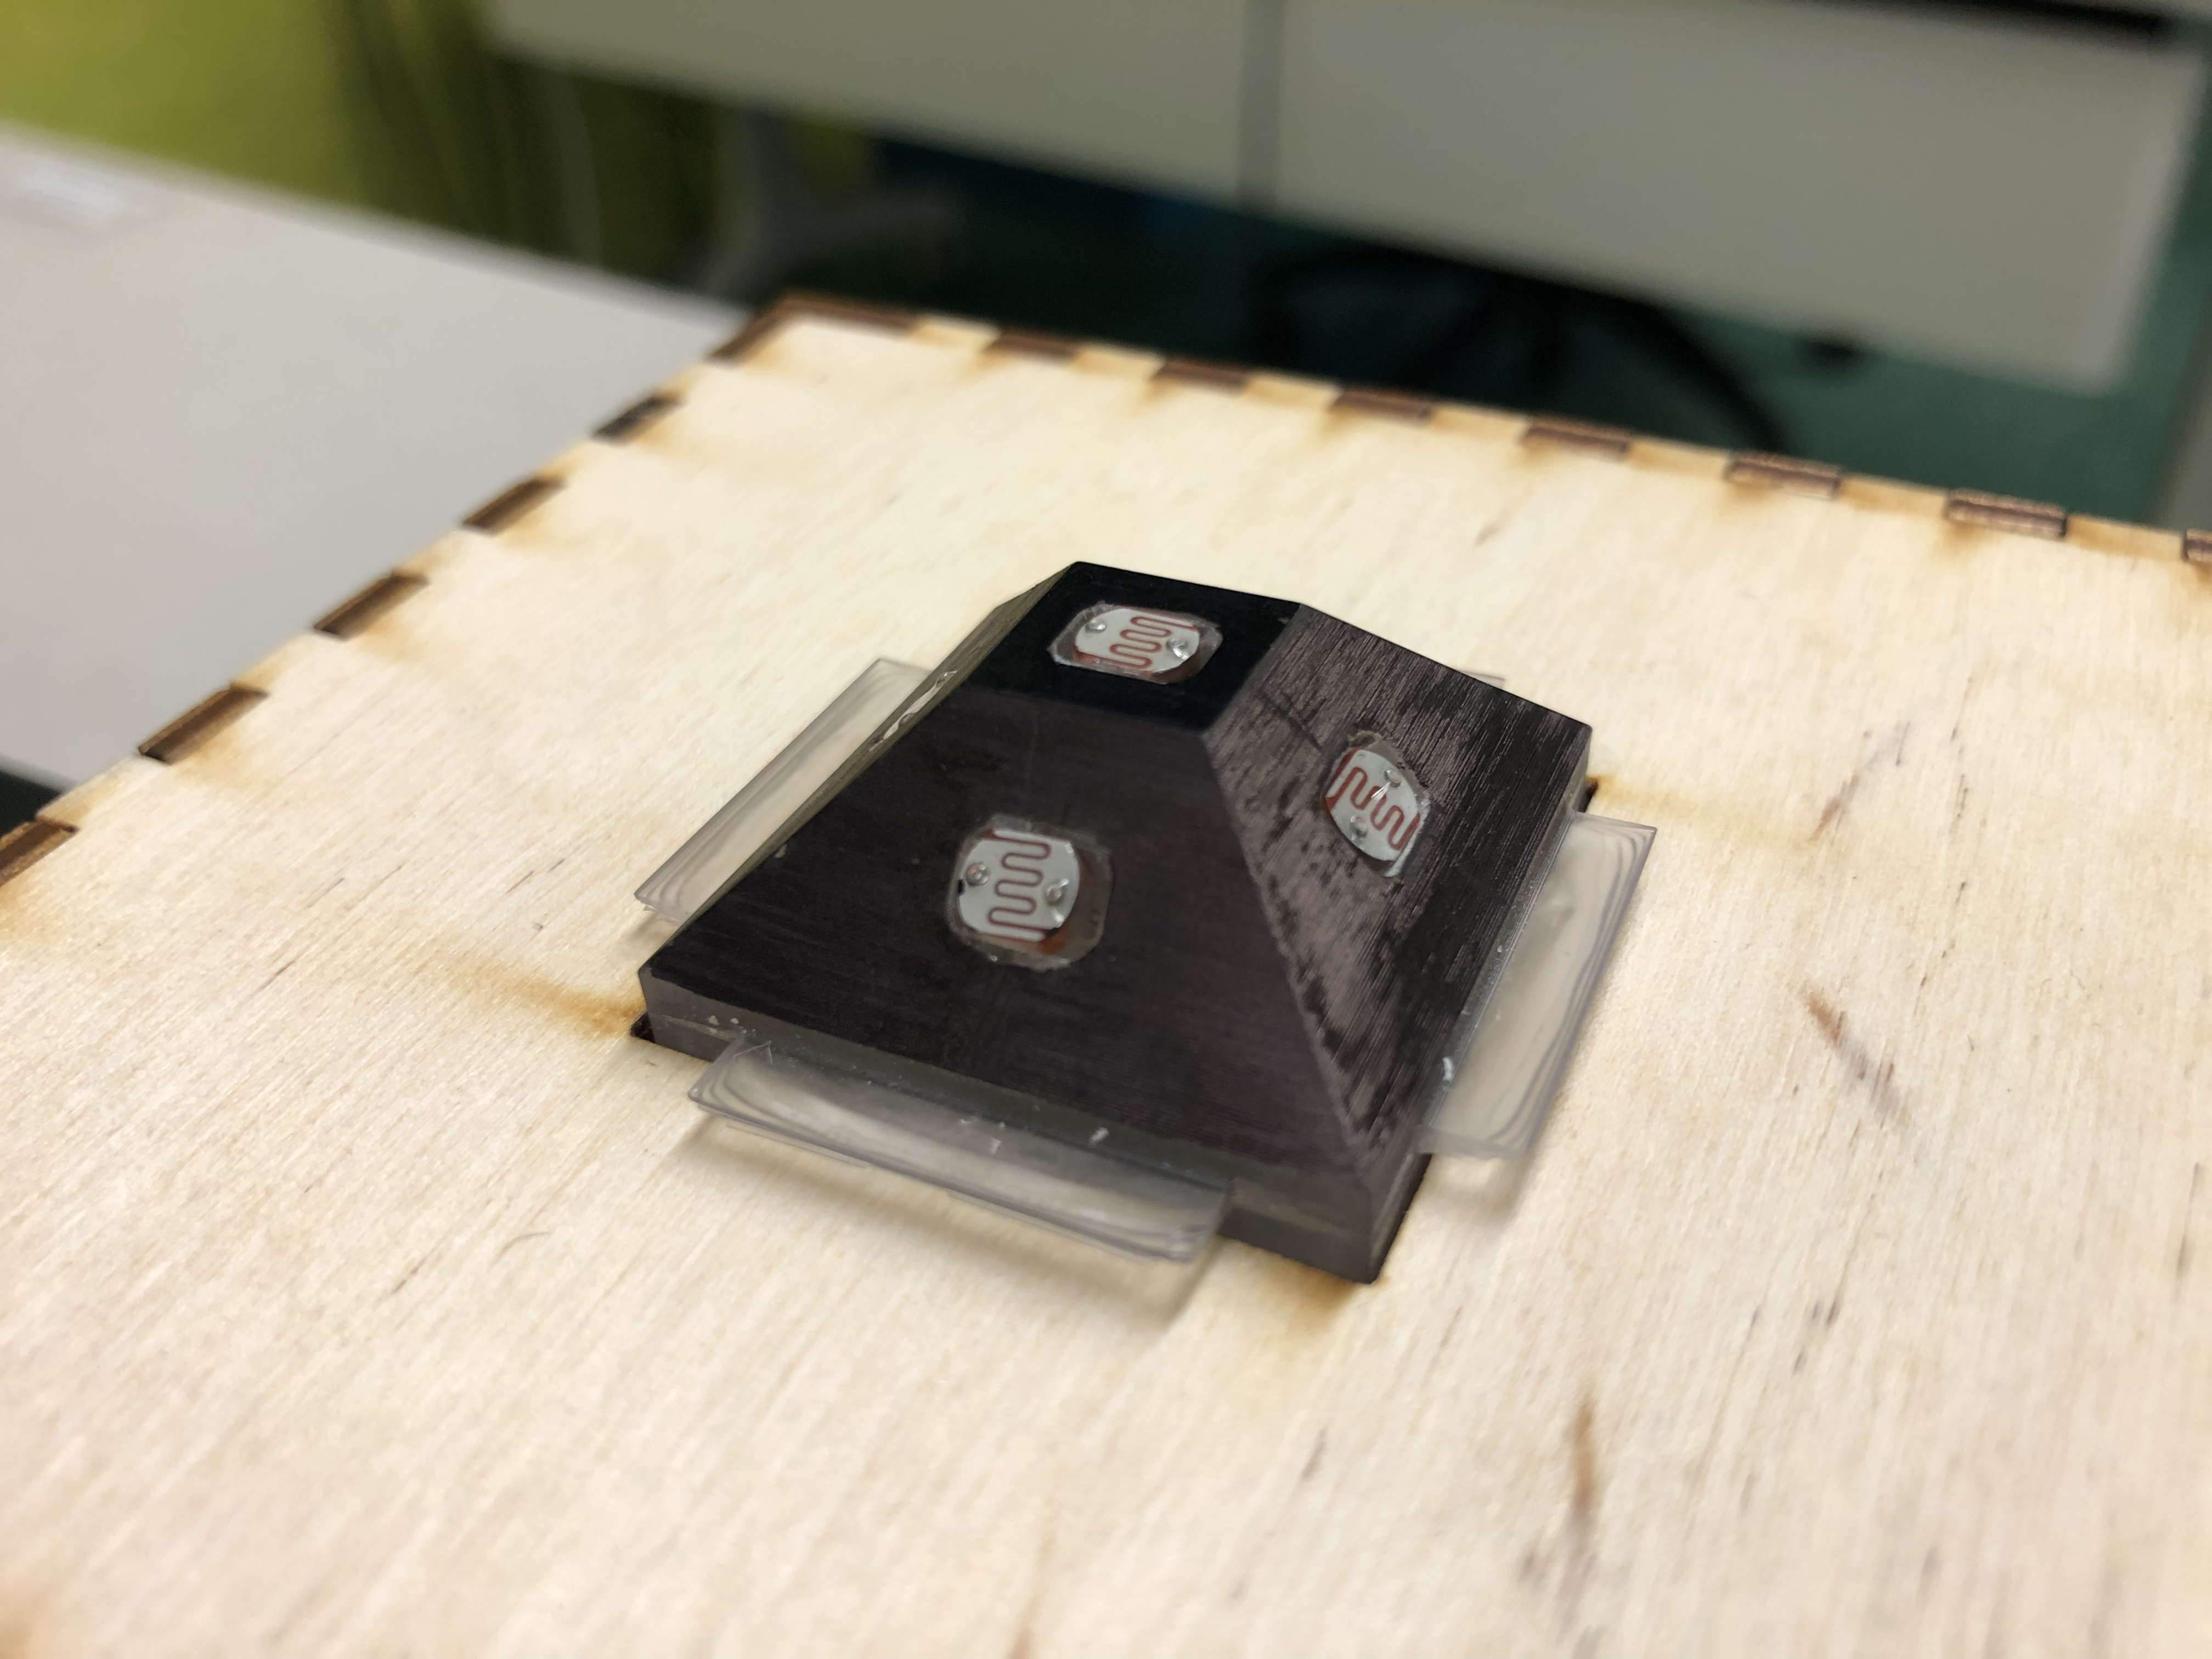
\includegraphics[width=0.8\linewidth]{figures/sun-sensor-painted.png}
	\caption{Sun sensor with painted exterior, mounted on the satellite.}
	\label{fig:sun-sensor-painted}
\end{figure}

The sun sensor successfully identified the direction of the flashlight, albeit with limited accuracy. I was not able characterize the accuracy with rigorous testing, but the output appeared to be within $15^\circ$ of the true direction. 

Once the satellite was assembled, I tested more code that controlled the rotation of the satellite stand and solar panel. There was a large amount of noise in the measurement data, which caused a lot of jitter due to the motors constantly making small adjustments. This was resolved by applying a moving average filter to the estimated direction of the light source and making the servo rotation rate proportional to the pointing error. Furthermore, since the SG90 servos could only rotate $180^\circ$, some additional logic was needed to coordinate the solar panel and satellite rotation in order to allow pointing in any direction above horizontal. 

After the software adjustments were made, the satellite was able to correctly track a moving light source and points its solar panel toward the light. This was demonstrated in class during the final project demo. 


\section{Reflection}
\label{sec:reflection}

\textbf{Question 1}: \textit{Show us what you made for your final project.  Include at least two in-process photos and two final photos (or videos!) of your final project. Include a paragraph about what challenges you faced and what you are most proud of, and any ``ah ha'' moments of insight or breakthroughs.}

See this report for photos and documentation. I am definitely most proud of the sun sensor design - I did not expect my first iteration to work out so well, and I was even more surprised when the math also worked first try. However, I am also very proud of how my laser cutting skills improved over this project. For both the solar panel supports and the improved satellite stand, I was able to very quickly draft up my ideas in Inkscape and laser cut them. Previously, I would've had less confidence and spent a lot more time trying to work around the problem instead of coming up with a solution. 

A related ``ah ha'' moment was when I needed to redesign the satellite stand. I initially redesigned the stand to be much wider and wanted to 3D print it, but realized that it would take over seven hours with minimal infill. Luckily, I realized that laser cutting plywood was much cheaper and faster before I decided to commit to the print. 

\textbf{Question 2}: \textit{Write a paragraph about your intended goal. What was your goal for the project, what prompt did you choose? Do you think you successfully met that goal? When was there a time when that goal seemed hard to achieve and what did you do to overcome it? If you failed to meet your goal, how did you iterate your plan and what did you learn in that process? }

See this report for details.

\textbf{Question 3}: \textit{Are you happy with your final project? Is your final project meaningful to you? Why?}

I am quite happy with the final project. While there are many things I could improve as detailed in this report, I think I came up with and realized a cool project in the limited amount of time available. It's a culmination of skills that I had coming into this class (programming, electronics) with new skills that I learned (laser cutting, 3D/resin printing), along with a dash of concepts that I use in my Ph.D. research. 

\textbf{Question 4}: \textit{Reread your previous assignment reflections, then write about what was the most significant thing you have learned over the course of the semester. This is not a question about tool learning, but rather a question about yourself as a learner and maker. }

I think the most significant thing that I learned is to be generous with prototyping. In many of my past projects, I would spend a lot of time perfecting a design, then get just the right amount of materials to build it. This might have something to do with how aerospace systems engineering is taught, since you really don't want to spend hundreds of millions of dollars making something and scrapping it for the next iteration. Nowadays, we are even seeing a shift to rapid prototyping in the aerospace industry, and there really is no reason not to prototype quickly for small projects like this mock satellite. This is something that I will keep in mind for my projects in the future. 

\textbf{Question 5}: \textbf{Has this course spurred you to think about yourself differently? And/or future goals and interests in life? Do you consider yourself a maker? What does that mean to you now that it didn’t at the beginning of the semester? What does it mean to you to call yourself a maker (or not)? Who do you think should call themselves a maker? }

I think anyone who has an idea and seeks out ways to create their idea is a maker, so I would consider myself to be one as well. While this course hasn't changed my future goals and interests, I do think it's helped me realize that there are a lot of resources available for me to realize my interests. For a long time, I've wanted to make a board game, and after taking this course I have already begun to prototype the board and the pieces at the makerspace. 

\textbf{Grad-specific questions for Prompt 1}: 
\begin{itemize}[]
	\item What is the problem or issue in your area of study that your project addresses? 
	
	See Section~\ref{sec:intro}.
	
	\item How has this issue or problem negatively affected your area of study?
	
	See Section~\ref{sec:intro}.
	
	\item How did you test your project to see if it might help this issue?
	
	See Section~\ref{sec:testing}.
	
	\item In what ways was your test successful and what ways did it fail? 
	
	See Section~\ref{sec:testing}.
	
	\item If you were to improve your project and test it again, how might you do that?
	
	Some of these have been mentioned above, but I will mention them again for completeness.
	
	Beginning with the sun sensor, I would redesign the resin-printed housing to separate the photoresistor leads. I would use a non-translucent resin if possible, or paint the print before I attach electronics to it. I would make a PCB to avoid having to solder together resistors in a big mess of braided wires. 
	
	On the software side, I would more rigorously test the response of each photoresistor. For example, I could ensure that the lighting conditions are identical, and I could test the signal strength at different incidence angles to the light (right now, I am assuming the response is sinusoidal). Additionally, I could filter the measurements from the photoresistor instead of filtering the calculated angles, or maybe even apply some real control systems concepts.
	
	Structurally, I would improve the body of the satellite by making the panels more easily removable, so that all six faces could be mounted if desired. Right now, two of the panels are removed to make the electronics easily accessible, which would not be necessary if the panels themselves were easily removable. 
	
	Finally, I would like to wire the solar panel into the Arduino to make it self-powered. I did some testing and found that the single solar panel I have can only produce ~2.2V and ~0.2mA. However, with two larger panels and perhaps a more efficient computer, it would be possible to drive the entire system using sunlight alone. 
	
\end{itemize}



\FloatBarrier
\newpage
\section*{Appendix A}

\begin{lstlisting}
// REQUIRES the BasicLinearAlgebra library by Tom Stewart
#include <BasicLinearAlgebra.h>
#include <Servo.h>
#include <math.h>

using namespace BLA;

bool allowRotation = false;

const int pinW = A0;
const int pinC = A1;
const int pinN = A2;
const int pinS = A3;
const int pinE = A4;

const int delay_ms = 50;

const int baseServoPin = 9;
Servo baseServo;
float baseServoPos = 0;
float baseServoDesired = 0;
float baseServoTarget = 0;
const int baseServo_moving_window_size = 20;
const float baseServo_gain = 0.08;

const int panelServoPin = 10;
Servo panelServo;
float panelServoPos = 90;
float panelServoDesired = 90;
float panelServoTarget = 90;
const int panelServo_moving_window_size = 20;
const float panelServo_gain = 0.08;

const float Nmax = 600;
const float Smax = 500;
const float Emax = 600;
const float Wmax = 600;
const float Cmax = 600;

Matrix<5,3> A = {0, 1/sqrt(2), 1/sqrt(2),  // N
                 0, -1/sqrt(2), 1/sqrt(2), // S
                 1/sqrt(2), 0, 1/sqrt(2),  // E
                 -1/sqrt(2), 0, 1/sqrt(2), // W
                 0, 0, 1};
Matrix<3,5> AT = ~A;
Matrix<3,3> AtAinv = AT*A;
bool is_nonsingular = Invert(AtAinv);
Matrix<3,5> normalMat = AtAinv*AT;

Matrix<5,1> meas;
Matrix<3,1> sunDir;

float ra = 0;
float dec = 0;

void setup() {
  Serial.begin(9600);
  baseServo.attach(baseServoPin);
  panelServo.attach(panelServoPin);
}

void loop() {
  // measurements
  float valN = analogRead(pinN);
  float valS = analogRead(pinS);
  float valE = analogRead(pinE);
  float valW = analogRead(pinW);
  float valC = analogRead(pinC);

  // disable/enable rotation based on top signal
  if (valN < 20) {
    allowRotation = !allowRotation;
    delay(1000);
  }

  // compute sun angle
  meas = {valN/Nmax, valS/Smax, valE/Emax, valW/Wmax, valC/Cmax};
  sunDir = normalMat * meas;
  float mag = sqrt(sunDir(0)*sunDir(0)+sunDir(1)*sunDir(1)+sunDir(2)*sunDir(2));
  sunDir /= mag;
  ra = atan2(sunDir(1),sunDir(0)) / PI * 180;
  dec = asin(sunDir(2)) / PI * 180;
  
  // set satelite and solar panel angles
  baseServoDesired = boundAngle(baseServoPos + ra);
  if (baseServoDesired < 0) {
    baseServoDesired += 180;
    panelServoDesired = 90 - (90-dec);
  } else {
    panelServoDesired = 90 + (90-dec);
  }
  baseServoDesired = boundServoPosition(baseServoDesired);
  panelServoDesired = boundServoPosition(panelServoDesired);

  // smoothing
  baseServoTarget = baseServoTarget * (1.0 - 1.0/baseServo_moving_window_size);
  baseServoTarget += baseServoDesired / baseServo_moving_window_size;
  panelServoTarget = panelServoTarget * (1.0 - 1.0/panelServo_moving_window_size);
  panelServoTarget += panelServoDesired / panelServo_moving_window_size;

  // set rotation
  baseServoPos += baseServo_gain * (baseServoTarget - baseServoPos);
  panelServoPos += panelServo_gain * (panelServoTarget - panelServoPos);
  baseServoPos = boundServoPosition(baseServoPos);
  panelServoPos = boundServoPosition(panelServoPos);

  // command rotation
  if (allowRotation) {
    baseServo.write(baseServoPos);
    panelServo.write(panelServoPos);
  }

  delay(delay_ms);
}

float boundServoPosition(float servoPos) {
  if (servoPos > 180) { return 180; } 
  if (servoPos < 0)   { return 0; }
  return servoPos;
}

float boundAngle(float ang) {
  return fmod(ang+180, 360) - 180;
}

\end{lstlisting}